\chapter{Concepts}
	\section{Packages}
		The software is split into two parent packages which themselves are split into
		sub packages. Figure \ref{fig:designPackages} shows those packages. One of
		the main package is \verb~HsrOrderApp~ comprising of everything from 
		the sample order application. This is specific code, including generated classes.
		The second main package is \verb~STORM~ and comprises of code which is not specific to
		the sample implementation. This makes it possible to distribute the \verb~STORM~ code
		independently.
	
		\begin{figure}[htb]
			\begin{center}
				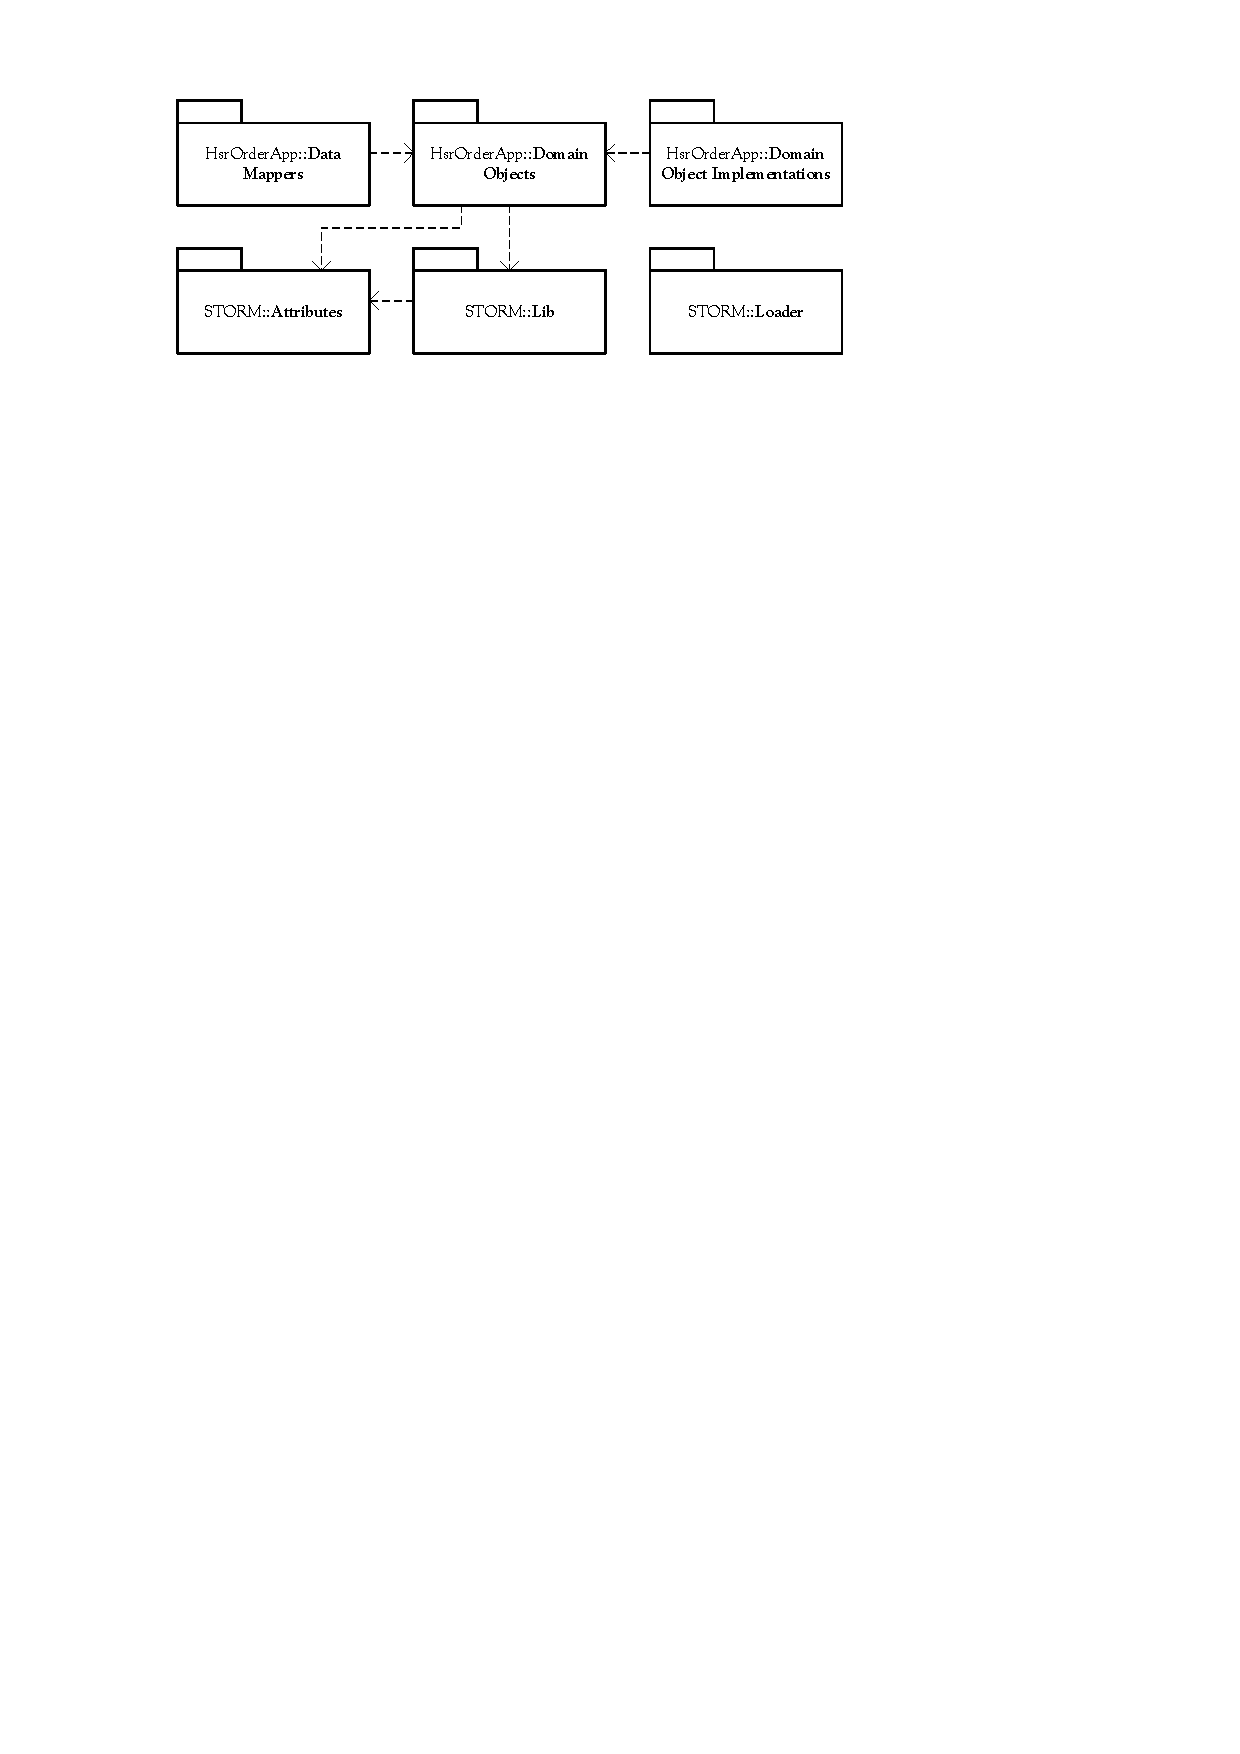
\includegraphics{./files/inc/figures/designPackages}
				\caption{\label{fig:designPackages} Software Packages}
			\end{center}
		\end{figure}
		
		The \verb~HsrOrderApp::Domain Objects~ package contains all abstract classes. These classes
		are needed to generate the mapping code. This is the starting point to write an application.
		The other two packages in \verb~HsrOrderApp::~ contain only generated code. This code
		is split into implementations of the domain objects and the mapping code for each domain
		object.
		
		The more important packages are \verb~STORM::~. The \verb~::Attribute~ package contains
		all custom attributes. This includes attributes which are used internally only by \textit{STORM} and 
		attributes which can be used to attribute abstract classes. All these attributes are listed in section 
		\ref{sec:attributes}. The package \verb~::Lib~ contains all generic classes which \textit{STORM}
		provides. At last, the \verb~::Loader~ package contains the \verb~AssemblyLoader~ and other classes
		related to CodeSmith.
		
		The \verb~STORM::Lib~ package is the core of the \textit{STORM} framework. Figure \ref{fig:designLibConcept}
		shows a conceptional model of this package. Some classes are generic and only used
		by the classes in the domain object. In the following sections, the different concepts
		are described. 
		
		\begin{sidewaysfigure}[htbp]
			\begin{center}
			\thispagestyle{plain}
				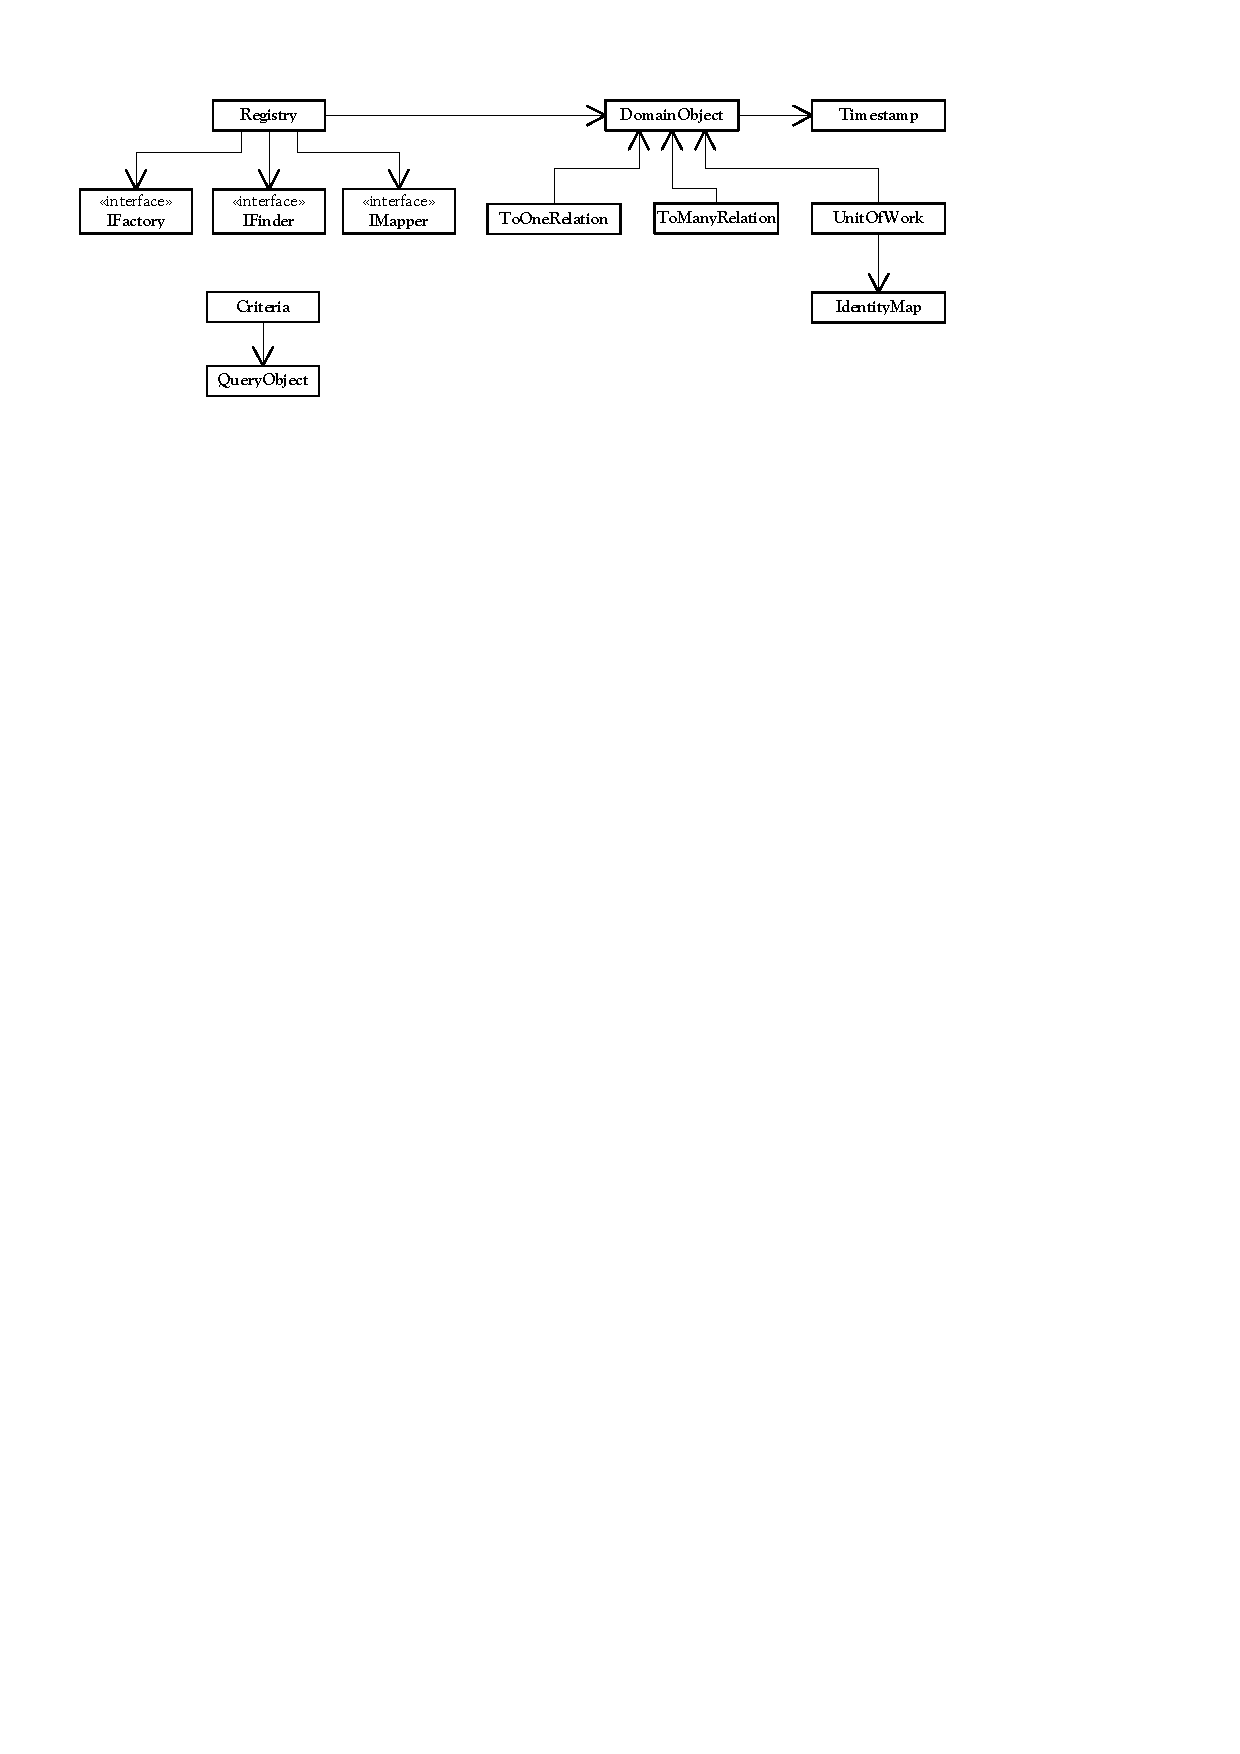
\includegraphics{./files/inc/figures/DesignLibConcept}
				\caption{\label{fig:designLibConcept} Conceptional Model of the STORM::Lib Package}
			\end{center}
		\end{sidewaysfigure}

				
	\section{Registry}
		As soon as an application starts, it must call the \verb~Registry~'s \verb~init()~ function.
		This function searches through all assemblies of the currently executed program and stores
		the type information of all domain object and mapper implementations in hashtables. These
		hashtables are used later to retrieve the appropriate implementation or mapper for a given
		type. Because we cannot know the type of implementations and mappers at design time, only
		interfaces are returned. This interfaces can be casted by the caller.
		The usage of the \verb~Registry~ is described in the following sections. Figure 
		\ref{fig:designRegistryAndInterfaces}	shows the registry class and the interfaces which are used
		in this context.
		
		\begin{figure}[htb]
			\begin{center}
				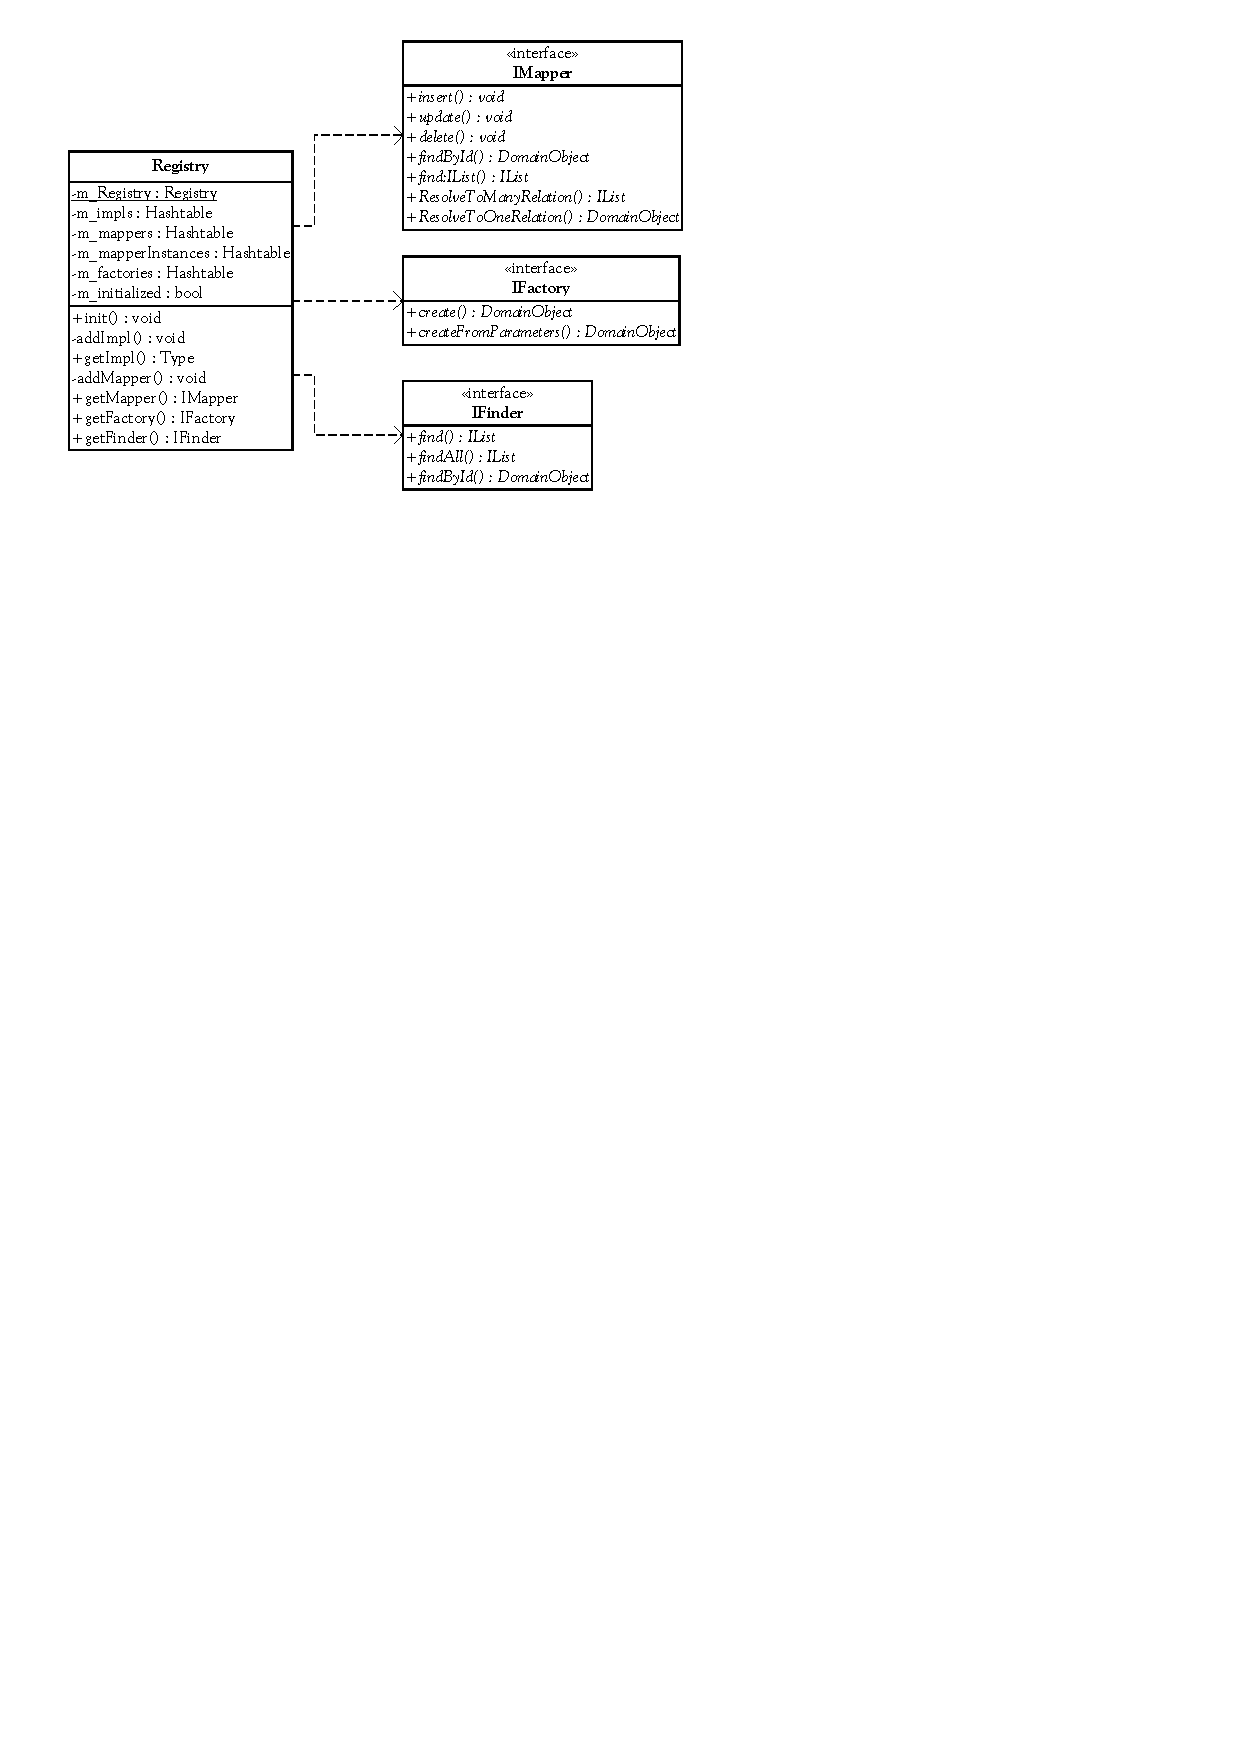
\includegraphics{./files/inc/figures/DesignRegistryAndInterfaces}
				\caption{\label{fig:designRegistryAndInterfaces} Registry and depending Interfaces}
			\end{center}
		\end{figure}
		
	\section{Unit of Work}
		A key concept in \textit{STORM} is the use of a \textit{Unit of Work} pattern. This pattern has
		already been described in section \ref{subsec:unitOfWork}. A UnitOfWork manages database
		connections and is responsible to execute database operations in the right order.
		
		Every time a new object is created, that object registers itself in the UnitOfWork as new.
		Similarly, if an object has been changed or deleted, that object registers itself as either
		dirty or removed.
		The UnitOfWork stores all this and executes the appropriate operations in the right order upon
		a commit request. If an object is transferred from the database, this object is registered as
		clean.
		
		Connections are handled through a \verb~Transaction~ object. Every time the UnitOfWork
		receives a commit request, it starts a new transaction. After all commands are executed,
		the transaction is closed. This is related to the locking mechanisms described in 
		section \ref{sec:lockingMechanisms}. Also the lifetime of a UnitOfWork has already been
		described in section \ref{sec:objectLifetime}.
		
	\section{Factory}
	\label{sec:Factory}
		As mentioned in chapter \ref{cha:designConsiderations}, it is important to avoid dependencies
		between generated and non-generated code. The solution is to use the \textit{Factory Method} pattern.
		In the case of \textit{STORM}, this means that whenever a new object is created, it must be 
		handled through the \verb~Registry~. This is somewhat more complicated but the most proper
		solution for it. For example, if a client wants to create a new \verb~Person~, it needs a
		constructor for it. If this constructor was declared in the abstract class, it would be
		of no use because abstract classes cannot be instantiated. And because of the dependency
		problem, a constructor in the domain object implementation cannot be called directly. But again, in order
		to create a new \verb~Person~, we need to call a constructor.
		
		The solution is to declare an internal class in the abstract domain object class and to parameterise
		it with the Factory attribute. This, for a \verb~Person~, would look like Listing
		\ref{lst:factoryClass}.
		
		\begin{lstlisting}[float=htb,language={[Sharp]C},caption=Defining a Factory Class,
		label=lst:factoryClass]
public abstract class Person : DomainObject
{
	[Factory]
	public abstract class PersonFactory
	{
		public abstract Person createPerson(
			[ParameterDef("PersonName")] string name,
			[ParameterDef("Password")] string password);
	}
}
		\end{lstlisting}
		
		Out of this declaration, a \verb~FactoryImpl~ and a static Property are generated 
		in the domain object implementation. When now a \verb~Person~ object should be created, the client can
		call the \verb~Registry~ for an appropriate FactoryImpl object. On this FactoryImpl object,
		the declared constructor can be called. Such a call would look like:
		\begin{Verbatim}
Person newPerson =
  ((Person.PersonFactory)Registry.Instance.getFactory(typeof(Person)))
  .createPerson("Jack", "password");
		\end{Verbatim}
		
		With this mechanism, there is no dependency between object which should not be. The drawback
		is that the usage is somewhat more complicated.
		
		Even if the Factory declaration in the abstract class is omitted, a FactoryImpl and a
		static Property will be generated in the domain object implementation.
		This is because the \verb~IFactory~ interface declares two methods to create an object. These
		methods can be called without declaring a custom Factory class in the abstract class. Furthermore,
		they are needed internally by \textit{STORM} to create objects which has been loaded from
		the database but do not exist as in-memory objects.
		
	\section{Finder Methods}
		\subsection{Self Defined}
			Another problem occurs with finder methods. Depending on the object in question, the
			finder methods will look differently. For example, a client wants to be able to call
			a method which looks like: 
			\begin{Verbatim}
public IList findByNameAndPassword(string name, string password){...}
			\end{Verbatim}
			This would return a list containing \verb~person~ objects which match the given name and password.
			The question is where to declare this methods.
			The solution is similar to the factory described in the last section. Finder methods
			can be declared in the abstract class as methods of a class attributed with the 
			\hyperlink{FinderAttribute}{Finder} attribute.
			An	example of such a declaration is given in Listing \ref{lst:finderClass}.
				
			\begin{lstlisting}[float=htb,language={[Sharp]C},caption=Defining a Finder Class,
			label=lst:finderClass]
public abstract class Person : DomainObject
{
	[Finder]
	public abstract class PersonFinder
	{
		public abstract IList findByName([ParameterDef("Name")] string name);
		public abstract IList findByNameAndPassword(
			[ParameterDef("Name")] string name,
			[ParameterDef("Password")] string password);
	}
}
			\end{lstlisting}
		
		Now, if a client wants to call a finder method, it asks the registry for an appropriate 
		finder implementation. On the returned object, the method can be called. Such a call would
		look like:
			
			\begin{Verbatim}
ArrayList foundPersons = new ArrayList();
foundPersons = ((Person.PersonFinder)Registry.Instance.getFinder(typeof(Person)))
               .findByName("Jack");
			\end{Verbatim}
			
			Because a finder method must be independent from a specific object (we do not want
			to create an object just to be able to call a find method), the implementation
			differs from the factory implementation. To be more precise, the code for
			a finder method must be in a appropriate mapper implementation, e.g. in the
			\verb~PersonMapper~. As we can see later, this is only true for generic finder methods.
			The reason is the following problem: A client cannot call
			a method which is defined in the abstract class and implemented in the mapper implementation.
			That is because a mapper implementation is not inherited from the abstract class
			(in contrast to the domain object implementations).
			Therefore, an implementation of the finder
			methods must persist in the domain object implementation such that a client is
			able to call it.
			
			The next consideration is how to call the generic finder method in the mapper implementation
			from within the domain object implementation. The solution is to use a 
			\textit{Query Object} pattern. With a query object, every custom defined finder method
			can be converted to an appropriate query object which then can be passed to 
			a generic finder method in the mapper implementation. Generic finder methods are described
			in \ref{subsec:genericFinder}.
			
			Figure \ref{fig:designFind} is a sequence diagram showing this finding scenario.
			
			\begin{figure}[htb]
				\begin{center}
					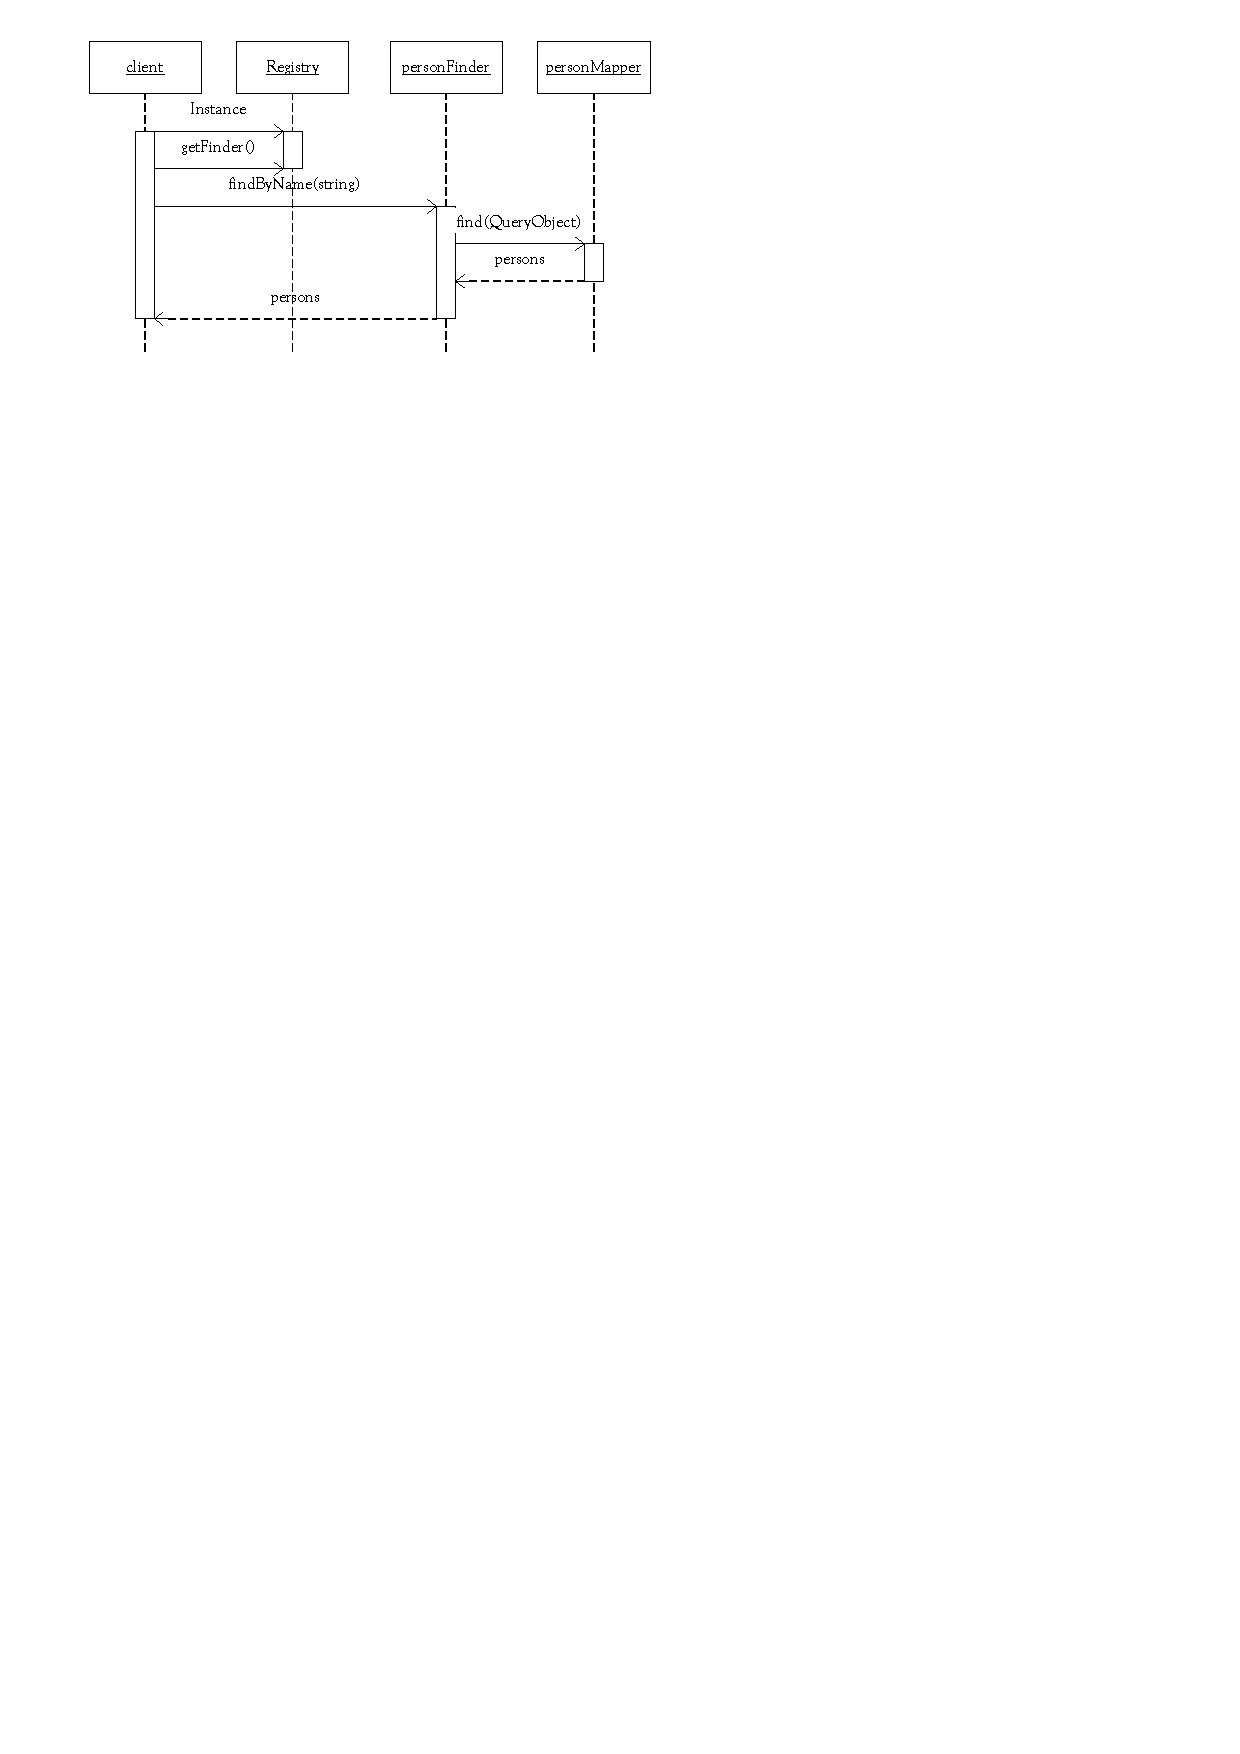
\includegraphics{./files/inc/figures/DesignFind}
					\caption{\label{fig:designFind}Finding objects with custom finder methods}
				\end{center}
			\end{figure}
			
		\subsection{Generic}
		\label{subsec:genericFinder}
			Because some finder methods are known and can apply to every type of object, not all finder methods must
			be self defined. Those methods which are generic have been made accessible through an interface (\verb~IFinder~).
			The implementation of these methods is in the mapper implementation class. 
			The following methods have been declared in the \verb~IFinder~ interface:
			\begin{Verbatim}
IList find(QueryObject qo);
IList findAll();
DomainObject findById(Key id);
			\end{Verbatim}
			
			The first method takes a \verb~queryObject~ as parameter. This object holds any number
			of \verb~criteria~ objects. If multiple \verb~criteria~ objects are added to a \verb~queryObject~, they
			are linked together with ``AND''. To stay with our person example, a call to find
			every person whose name is 'Jack' would look like:
			
			\begin{Verbatim}
QueryObject qo = new QueryObject();
qo.addCriteria(new Criteria(Criteria.Operator.Equal, "Name", "Jack"));

ArrayList foundPersons = new ArrayList();
foundPersons = Registry.Instance.getFinder(typeof(Person)).find(qo);
			\end{Verbatim}
			
			These makes it possible to form self defined find constructs through a \textit{Query Object}.
			The result is the same as to define a method in the abstract class but sometimes it is  more
			flexible to use. Figure \ref{fig:DesignQueryObjectAndCriteria} shows the 
			\verb~QueryObject~ class and its relation to \verb~Criteria~.
			
			The other two methods are self explaining and can be used accordingly.
			
			\begin{figure}[htb]
				\begin{center}
					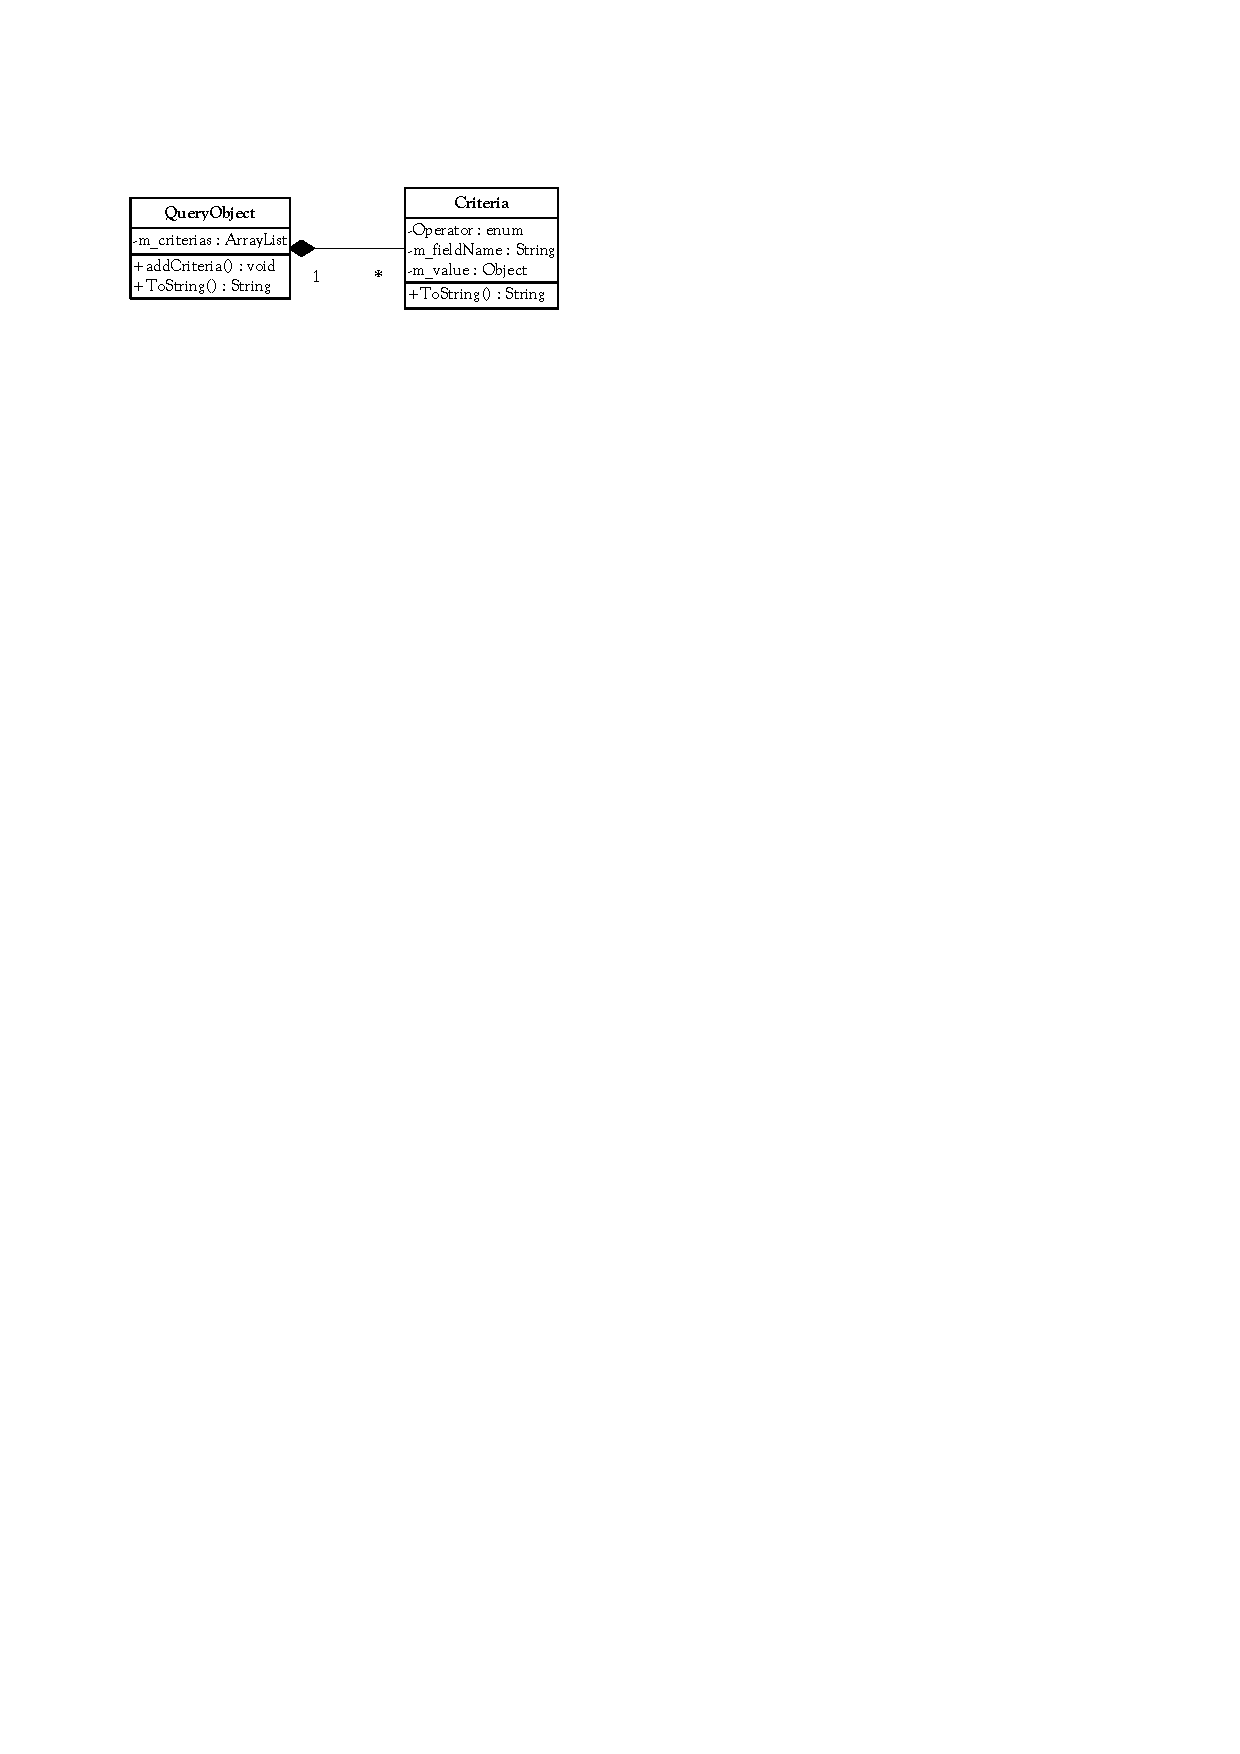
\includegraphics{./files/inc/figures/DesignQueryObjectAndCriteria}
					\caption{\label{fig:DesignQueryObjectAndCriteria}Relation between QueryObject and Criteria}
				\end{center}
			\end{figure}
			
	
	\section{Adder Methods}
		Adder methods are those which can be used to add related objects to the current object. For example,
		a \verb~person~ can have an adder method to add \verb~address~ objects which are related to
		the person (e.g. her/his addresses). This is different from creating and finding objects because an
		adder method must be called on the object itself, e.g. on a \verb~person~ object. This means,
		an object must be existing. Therefore, the only sensible place to have adder methods
		implemented is the domain object implementation.
		
		Adder methods are used in conjunction with \hyperlink{ToManyAttribute}{ToMany}
		relations. A code snippet from the abstract class \verb~Person~ is given in Listing
		\ref{lst:personAdder}. The example defines a ToMany relation and a belonging adder method.
		
		\begin{lstlisting}[float=htb,language={[Sharp]C},caption=Defining an Adder Method,
			label=lst:personAdder]
[ToMany(typeof(Order), "Person")]
public abstract IList Orders {get;}

[Adder("Orders", "Person")]
public abstract void addOrder(Order o);
		\end{lstlisting}
		
		The code for all adder methods is generated into the domain object implementation.
		For example, the resulting code for the adder method shown in \ref{lst:personAdder}
		looks like (exception handling is omitted):
		
		\begin{lstlisting}[float=htb,language={[Sharp]C},caption=Defining an Adder Method,
			label=lst:personAdderImpl]
public override void addOrder(Order o)
{
	if(o != null)
	{
		o.Person = this;
		m_Orders.Add(o);
	}
}
	\end{lstlisting}
	
	m\_Orders is an object of type ToManyRelation which holds all related objects. Adder methods
	could be generated automatically, but again, if they were, it would not possible to call
	those methods from a client. o.Person is the back reference from an order to a person.
	
	%----------
	\section{Data Flow}
		This section is about the work flow of \textit{STORM}. It covers and explains
		the most important flow scenarios. These are creating new objects, deleting objects and lazy load.
		
		\subsection{Create New Object}
			A new object is represented in an application with a new instance of a class. This
			instance is registered within the \textit{Unit of Work} as new. Whenever the \textit{Unit of Work} 
			receives a commit, this new class needs to be written to the database. For this, a new
			transaction is created after the commit is received. A transaction represents a database connection
			for a certain, limited time. In this case, a transaction is created at the beginning of the
			commit method and is closed at its end. For the time of this transaction, the database
			is exclusively locked. To actually write the new created object to the
			database, the specific mapper's \verb~insert()~ method is called. This method 
			writes the object to the database. The whole process is illustrated in Figure
			\ref{fig:designNewObject}.
			
			\begin{sidewaysfigure}[htb]
				\begin{center}
				\thispagestyle{plain}
					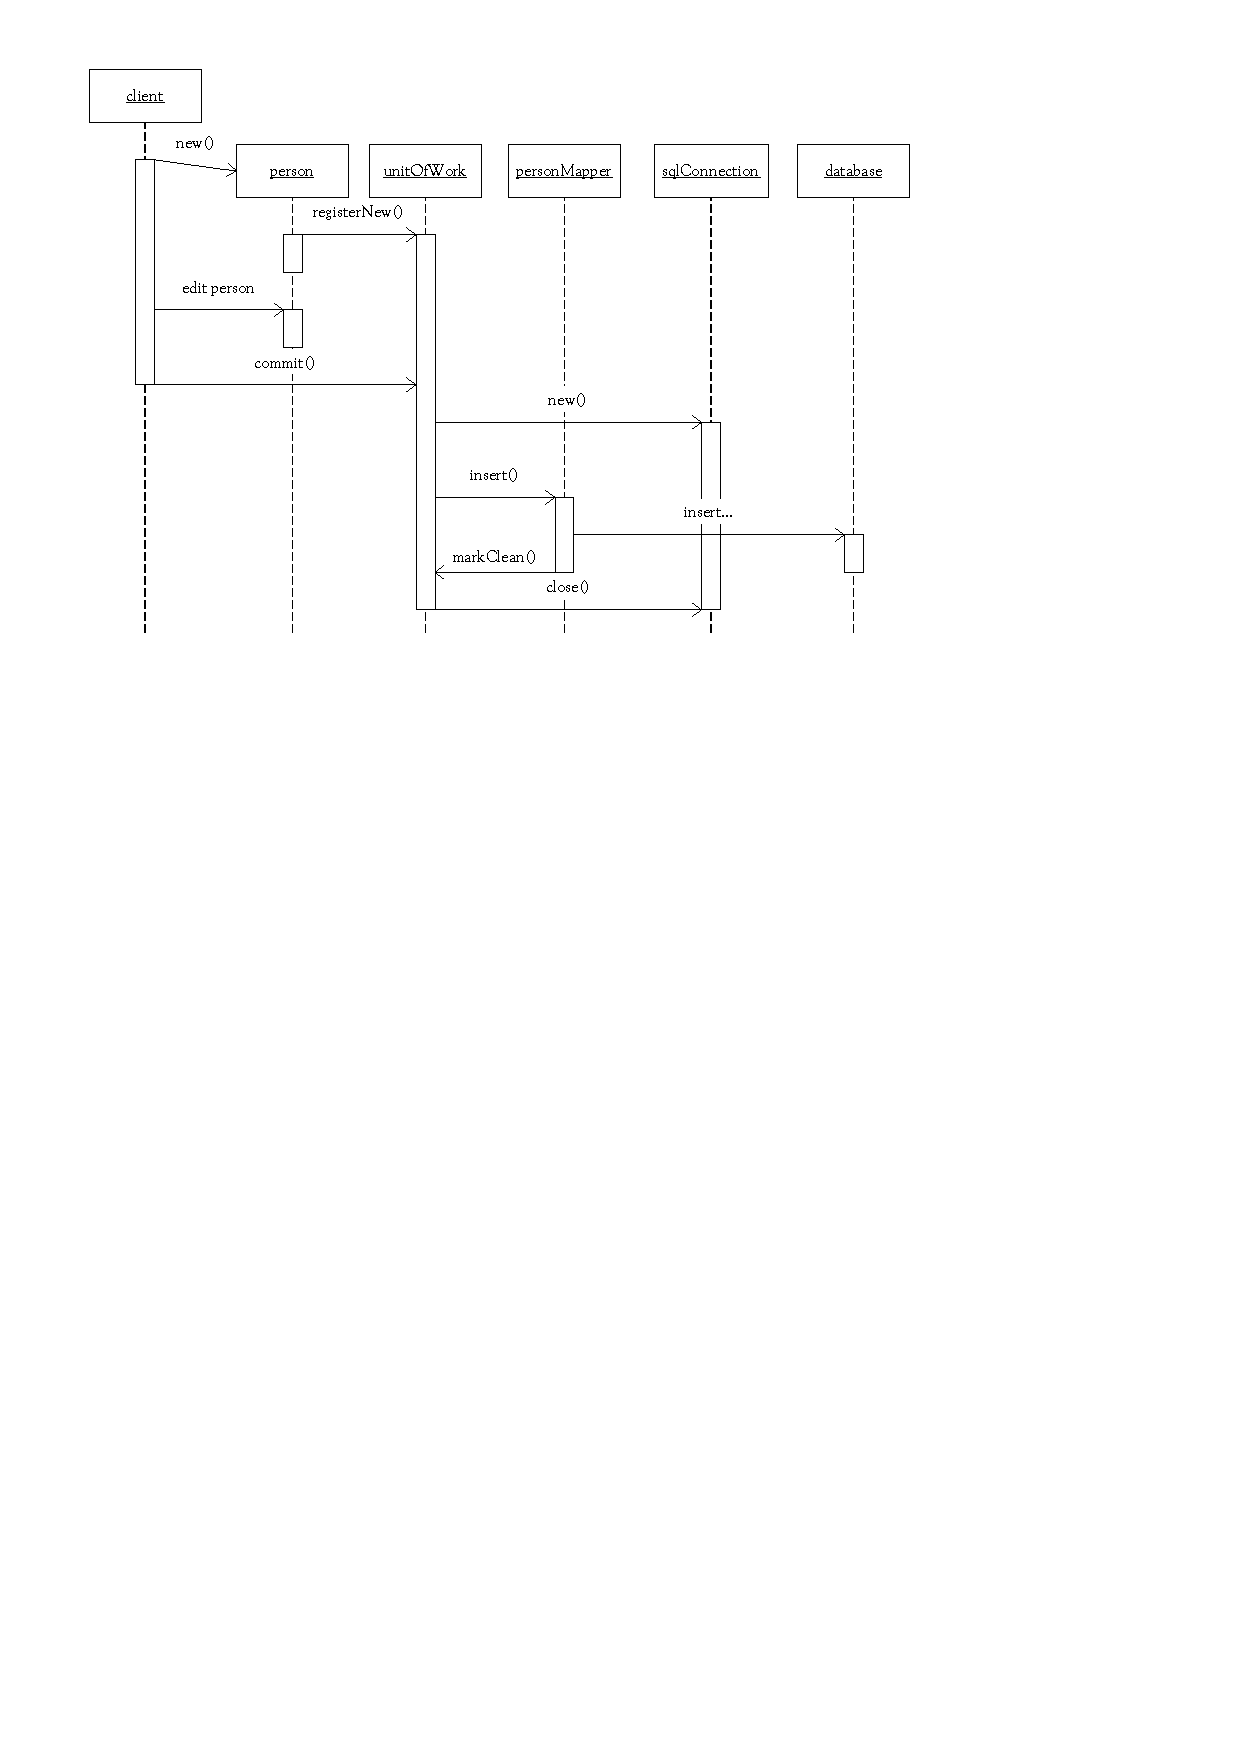
\includegraphics{./files/inc/figures/DesignNewObject}
					\caption{\label{fig:designNewObject} Creating a new Object}
				\end{center}
			\end{sidewaysfigure}

		\subsection{Lazy Load}
		\label{subsec:LazyLoad}
			Our object/relational mapper not only handles the mapping between classes and tables etc., it
			provides a mechanism to enhance performance. Vital to every application which transfers
			object over a network is to limit the number of remote calls. \textit{Lazy Load} provides
			a mechanism to handle this need. When talking about \textit{Lazy Load}, a few decisions need to be
			made before implementing a concrete solution. The most important concerns object lifetime. There are
			3 main ways which are as follows:
			\begin{enumerate}
				\item Whenever an object needs to be loaded, it will be fully loaded from the database,
							regardless of the fact if it had been already loaded before.
				\item	Before loading an object from the database, a class (see Identity Map \ref{subsec:identityMap}) which holds
							already transfered objects in a map is called to check if the object had been transferred before. 
							If so, the desired object is loaded	directly from this map instead of transferring it again. This
							sounds like a good alternative to the first mechanism but has the disadvantage of possible consistency
							errors. This leads to conflict resolution strategies which can be quite challenging to solve.
				\item	The third possibility is close to the second one except that an object's version field is compared
							with the version field on the database to check if the object is still up to date. If those versions
							match, the object from the map is loaded, otherwise the object will be reloaded from the
							database.
			\end{enumerate}
			The first strategy is the most simple to implement. It does not need an \textit{Identity Map} nor 
			\textit{Lazy Load}. Event though, it is not the most performant solution because objects are transferred
			more often. The second strategy would be, depending on the application though, more performant but much
			more complicated to implement. Additionally, it is not a good solution for code generation because
			conflict resolution strategies are very specific and can therefore not be generated automatically.
			For these reasons, we use the third strategy which should result in a good performance and a secure
			way to update objects. The process is illustrated in Figure \ref{fig:designLazyLoad}. It shows
			a find operation where all addresses for a person are searched.

			\begin{sidewaysfigure}[p]
				\begin{center}
					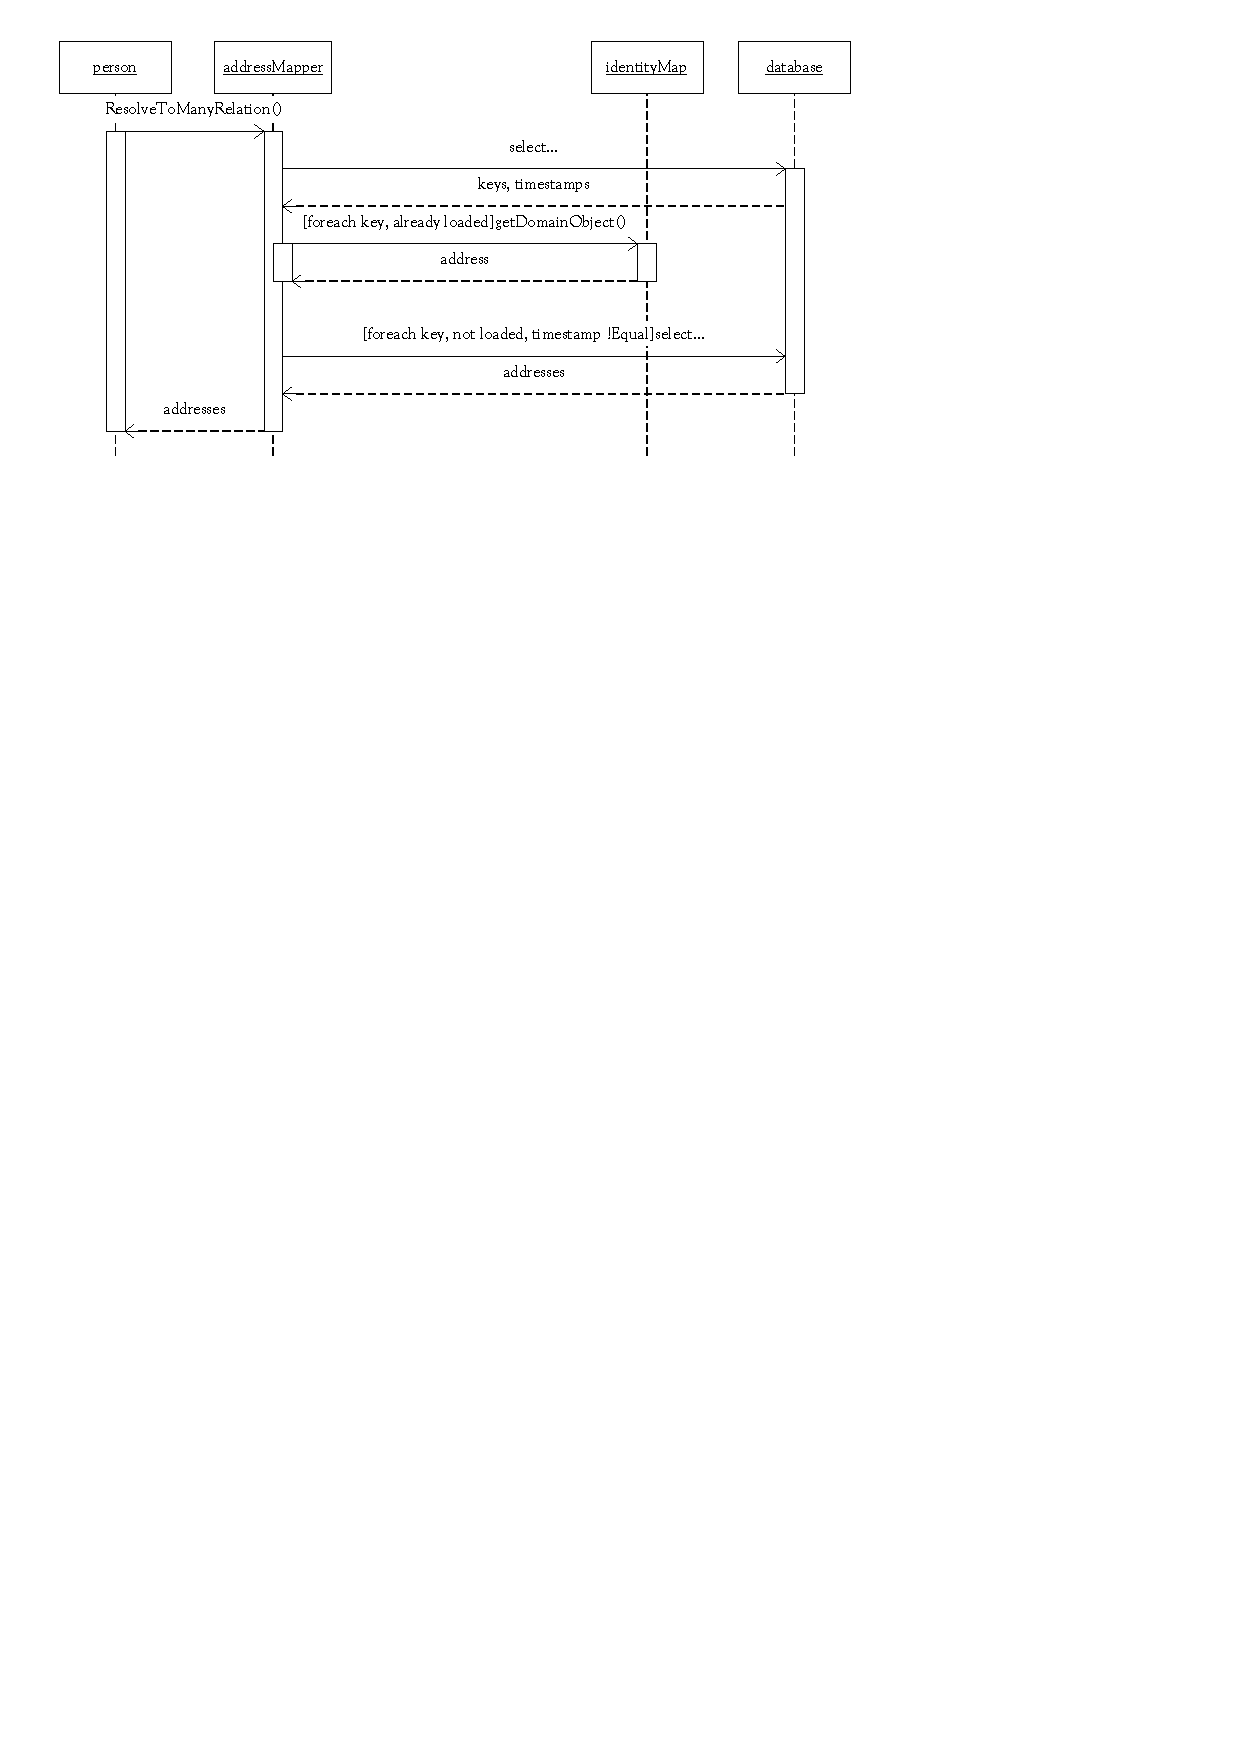
\includegraphics{./files/inc/figures/DesignLazyLoad}
					\caption{\label{fig:designLazyLoad} Lazy Load mechanism}
				\end{center}
			\end{sidewaysfigure}
			
		\subsection{Delete Object}
			Another scenario originates when an object (e.g. a Person) is deleted. It is not
			possible to just delete the person on the database because a person can have
			relations like addresses which has to be deleted first.
			In our example, this means to call the delete function on each address. The Address 
			will be marked as removed and registers itself in the UnitOfWork to be removed.
			After all addresses have been processed, the person
			itself can be registered to be removed. Because the \textit{Unit of Work} remembers
			the correct order, all addresses will be removed before the person is removed.
			Figure \ref{fig:designDelete} shows this procedure. \textit{Lazy Load}
			is also used to make sure that all objects are up to date but it is omitted in the
			sequence diagram.
						
			\begin{sidewaysfigure}[p]
				\begin{center}
					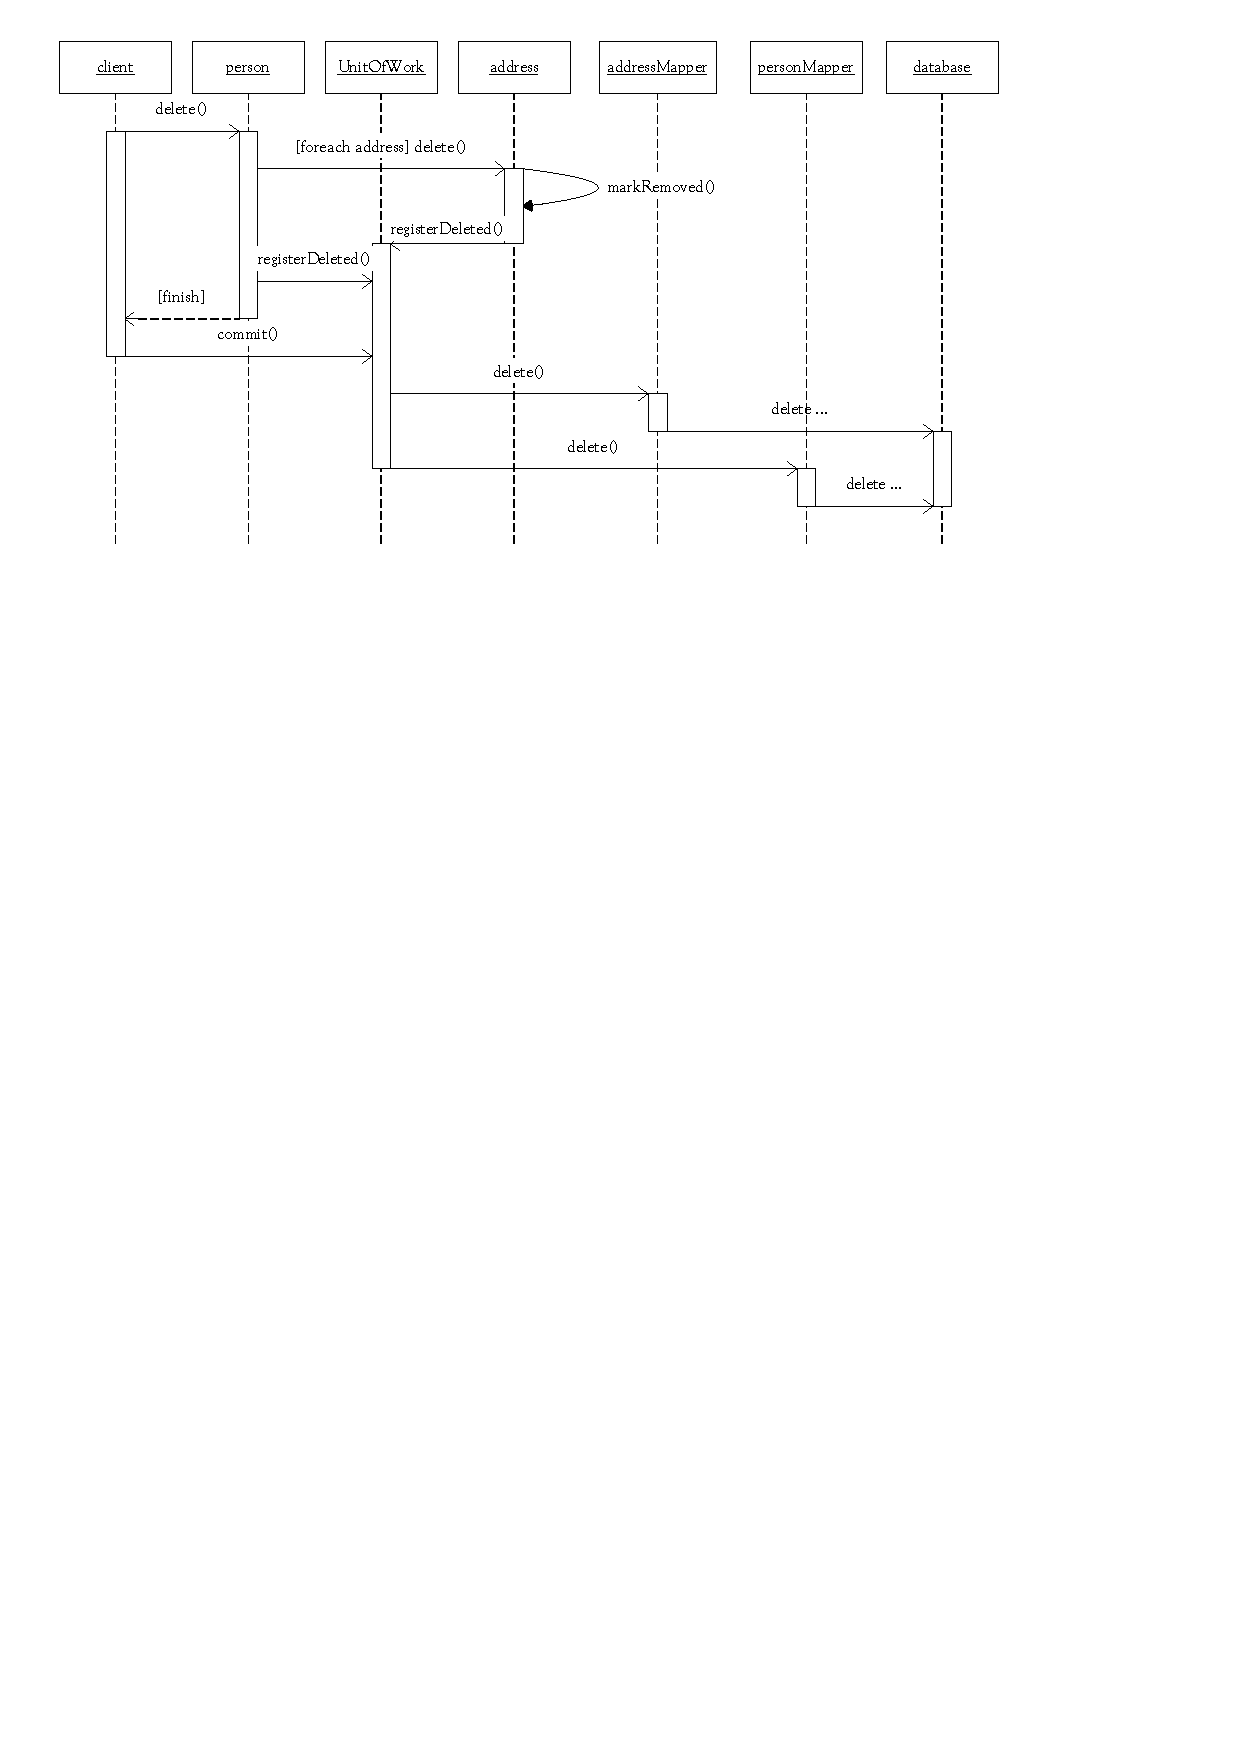
\includegraphics{./files/inc/figures/DesignDelete}
					\caption{\label{fig:designDelete} Delete an Object}
				\end{center}
			\end{sidewaysfigure}
			
	%----------
	\section{Attributes}
	\label{sec:attributes}
		Here is a list of all custom attributes which \textit{STORM} defines:
		
		\LTXtable{\linewidth}{./files/inc/tables/designAttributes}
		
		The following description list describes each attribute. This is only a short description
		meant as an overview.
		Parameter description is omitted.
		\begin{description}
			\item[Adder]
				Defines a method to add any objects to the current object. For example, it can be used
				to add an \verb~Address~ object to a \verb~Person~ object. This attribute is usually used
				for a \hyperlink{ToManyAttribute}{ToMany} relation. It is needed
				because an adder could not be called it it was generated automatically in the domain
				object implementation.
			\item[Column]
			\hypertarget{ColumnAttribute}{}
				Defines the mapping between a member variable and a column in the database. It is used for
				properties only. Out of these properties, the corresponding member variables are generated.
			\item[DomainObjectImpl]
			\hypertarget{DomainObjectImplAttribute}{}
				This is an internal only attribute. It must not be declared in an abstract class. Instead, it
				is automatically declared in the generated code and is used by the registry to know 
				which generated classes are to be treated as a domain object implementation and 
				should therefore be registered in the registry.
			\item[Factory]
			\hypertarget{FactoryAttribute}{}
				This attribute is used to specify the factory. It is used to attribute an abstract class declaration.
				Within this class, create methods can be specified. Out of this specification, constructors
				are generated which can be called from within a user written client program. A class specified with
				the Factory attribute must be enclosed by the main abstract class.
			\item[Finder]
			\hypertarget{FinderAttribute}{}
				Like the \hyperlink{FactoryAttribute}{Factory} attribute,
				this is an attribute which is used for an abstract class. Within this class, abstract methods
				can be declared. Out of these declaration, custom defined finder methods are generated.
			\item[GenerateCode]
				This attribute is used for every user defined, abstract class to indicate that
				code for this class should be generated. If omitted, the class will be completely
				ignored by \textit{STORM}.
			\item[MapperImpl]
				This is an internal only attribute. It must not be declared in an abstract class. Instead, it
				is automatically declared in the generated code and is used by the registry to know 
				which generated classes are to be treated as a mapper implementation and 
				should therefore be registered in the registry.
			\item[ParameterDef]
				This attribute is used in within the abstract \hyperlink{FactoryAttribute}{Factory} and
				\hyperlink{FinderAttribute}{Finder} classes. They define the mapping between
				parameters and the corresponding properties.
			\item[PrimaryKey]
			\hypertarget{PrimaryKeyAttribute}{}
				Declares that the primary key in the database is represented by this property. This attribute
				must always be used in conjunction with a \hyperlink{ColumnAttribute}{Column} attribute.
			\item[Table]
			\hypertarget{TableAttribute}{}
				This attribute maps the whole class to a table in the database. At this time, one class
				can only map to exactly one table. Additionally, this attribute declares if the
				\hyperlink{PrimaryKeyAttribute}{PrimaryKey} is a surrogate key or a compound key.
			\item[ToMany]
			\hypertarget{ToManyAttribute}{}
				Declares a relation to a collection of other objects. This maps a 1:n relation in the
				database to in-memory objects.
			\item[ToOne]
			\hypertarget{ToOneAttribute}{}
				Declares a relation to another object. This maps a 1:1 relation in the database to in-memory
				objects. It must be used to specify the back link to a \hyperlink{ToManyAttribute}{ToMany} relation.
				For example, if a \verb~Person~ specifies a \hyperlink{ToManyAttribute}{ToMany} relation to
				\verb~Address~, \verb~Address~ must declare a ToOne relation back to \verb~Person~.
				This attribute is always used in conjunction with a \hyperlink{ColumnAttribute}{Column} attribute.
			\item[VersionField]
				Specifies a version field in the database. This field is a auto-generated field of the data type
				\verb~timestamp~ and is used to check if the in-memory object is in sync with the database object.
		\end{description}
		